
Die üblichste Methode um eine Frequenzanalyse über ein längeres Signal anzuwenden ist die  Kurzzeit-Fourier-Transformation oder auch short-time Fourier transform, kurz STFT. Bei dieser Methode wird das Signal in kleine abschnitte zerhackt und bei jedem dieser Signalstücke eine Fourier-Transformation angwendet. Wobei üblicherweise die Fourier-Transformation in Anwendungen mit dem schnellen Fourier-Transformations Algorhytmus berechnet wird. Was dieses Verfahren schnell rechenbar macht.

\subsection{Zeitkontinuierliche STFT}
Das Signal wird mit einer Fensterfunktion $\omega $ multipliziert. $\omega $ ist nur in dem gewählten Zeitbereich ungleich 0. Es gibt eine ganze Reihe an Fensterfunktionen zu den üblichsten gehören folgende:

\begin{itemize}
	\item Rechtecksfunktion
	\item Von-Hann-Fenster
	\item Gauss-Fenster
	\item B-spline
	\item Blackman
\end{itemize}


Das Produkt des Signals $x$ mit der Fensterfunktion $\omega $ liefert uns also eine neue Funktion die im Bereich ausserhalb des Fensters alle Werte auf null gesetzt hat. In der Anwendung sind diese Fenster meistens ein wenig überlappend damit kein Datenverlust entsteht. \\
Die Zeitkontiunierliche STFT ist  gegeben als:
\begin{equation}
X(\tau, \omega)=\int_{-\infty}^{\infty} x(t) w(t-\tau) e^{-j \omega t} dt
\end{equation}
mit der Kreisfrequenz  $\omega $

\subsection{Zeitdiskrete STFT}
Bei der Zeitdiskreten STFT liegt das Signal in einzelnen Abtastwerten vor. Diese Abtastwerte werden dann durch die Fensterfunktionen in einzelne Abschnitte unterteilt. \\
Die diskrete STFT ist gegeben als:
\begin{equation}
X(m, \omega)=\sum_{n=-\infty}^{\infty} x[n] w[n-m] e^{-j \omega n}
\end{equation}

\subsection{Verhalten der STFT}
In der Abbildung \ref{fig:stftauf} kann man die grafische Darstellung der Zeit-Frequenz-Auflösung sehen. Bei gleichbleibendem Flächeninhalt der einzelnen Rechtecke ist auf der linken Seite eine feinere Zeitauflösung zu sehen. Wobei Rechts eine bessere Frequenzauflösung aufweist. Dies wird durch die Küpfmüllerschen Unbestimmtheitsrelation welche besagt, dass die Zeitdauer und die Bandbreite eines Signals nicht gleichzeitig beliebig klein werden können. Dies ist eine zur Heisenbergschen Unschärferelation analoge Aussage welche auf die Nachrichtentechnik übernommen wurde.

\begin{figure}[!ht]
	\centering
	\scalebox{.75}{
	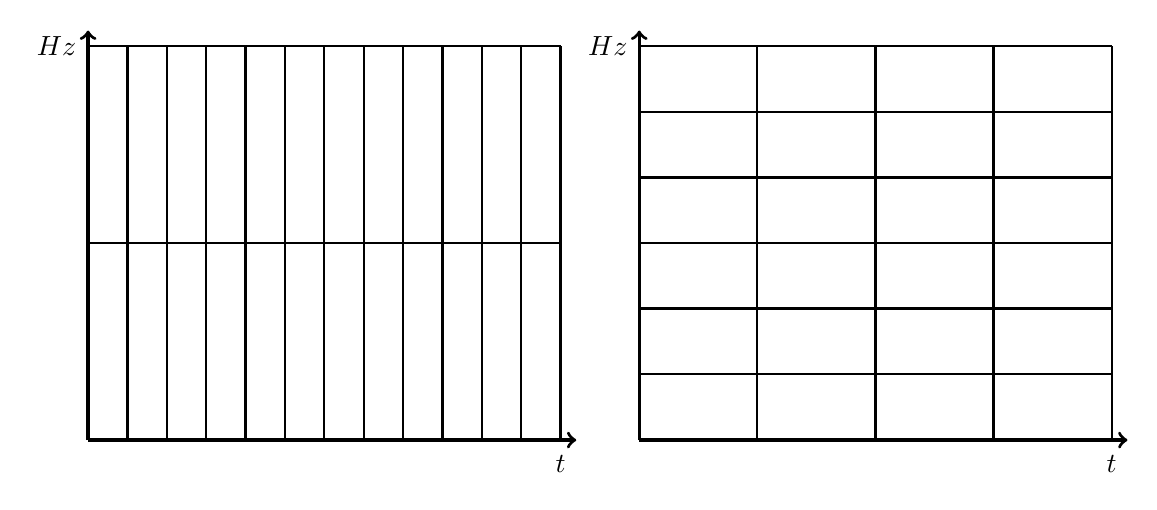
\begin{tikzpicture}
		\draw (6,-5.3) node{$t$};
		\draw (-0.4,0) node{$Hz$};
		\draw[->, very thick] (0,-5)--(0,0.2);
		\draw[->, very thick] (0,-5)--(6.2,-5);
		
		\draw[thick] (0,-0)--(6,-0);
		\draw[thick] (0,-2.5)--(6,-2.5);
		
		\draw[thick] (0.5,-5)--(0.5,0);
		\draw[thick] (1,-5)--(1,0);
		\draw[thick] (1.5,-5)--(1.5,0);
		\draw[thick] (2,-5)--(2,0);
		\draw[thick] (2.5,-5)--(2.5,0);
		\draw[thick] (3,-5)--(3,0);
		\draw[thick] (3.5,-5)--(3.5,0);
		\draw[thick] (4,-5)--(4,0);
		\draw[thick] (4.5,-5)--(4.5,0);
		\draw[thick] (5,-5)--(5,0);
		\draw[thick] (5.5,-5)--(5.5,0);
		\draw[thick] (6,-5)--(6,0);
		
		\draw (13,-5.3) node{$t$};
		\draw (6.6,0) node{$Hz$};
		\draw[->, very thick] (7,-5)--(7,0.2);
		\draw[->, very thick] (7,-5)--(13.2,-5);
		
		\draw[thick] (7,-0)--(13,-0);
		\draw[thick] (7,-0.833)--(13,-0.833);
		\draw[thick] (7,-1.666)--(13,-1.666);
		\draw[thick] (7,-2.499)--(13,-2.499);
		\draw[thick] (7,-3.33)--(13,-3.33);
		\draw[thick] (7,-4.166)--(13,-4.166);
		
		\draw[thick] (8.5,-5)--(8.5,0);
		\draw[thick] (10,-5)--(10,0);
		\draw[thick] (11.5,-5)--(11.5,0);
		\draw[thick] (13,-5)--(13,0);
	\end{tikzpicture}
	}
	\caption{STFT Zeit-Frequenz-Auflösung}\label{fig:stftauf}
	
\end{figure}

Dieses Unschärfe kann man nun bei einer STFT-Analyse \ref{tab:STFTtab} beobachten. Die Unschärfe wird gut erkennbar wenn man ein beliebiges Signal mit zeitlich verschieden langen Fenstern Analysiert. Wobei bei diskreten werten dies direkt in anzahl Samples pro Fenster gesehen werden muss.\\
 
Um das zu veranschaulichen betrachten wir einen Frequensweep von 0 bis 400$[Hz]$ der mit einem viel langsameren cosinus moduliert wurde. Danach wurden das Signal mit vier verschiednen Fensterbreiten des Types Blackman Analysiert.\\

Wobei das Blackman Fenster wie Folgt definiert ist:
\begin{equation}
w[n]=a_{0}-a_{1} \cos \left(\frac{2 \pi n}{N}\right)+a_{2} \cos \left(\frac{4 \pi n}{N}\right)
\end{equation} 
\begin{equation}
a_{0}=\frac{1-\alpha}{2} ; \quad a_{1}=\frac{1}{2} ; \quad a_{2}=\frac{\alpha}{2}
\end{equation}


\begin{table}[!ht]
	\centering
	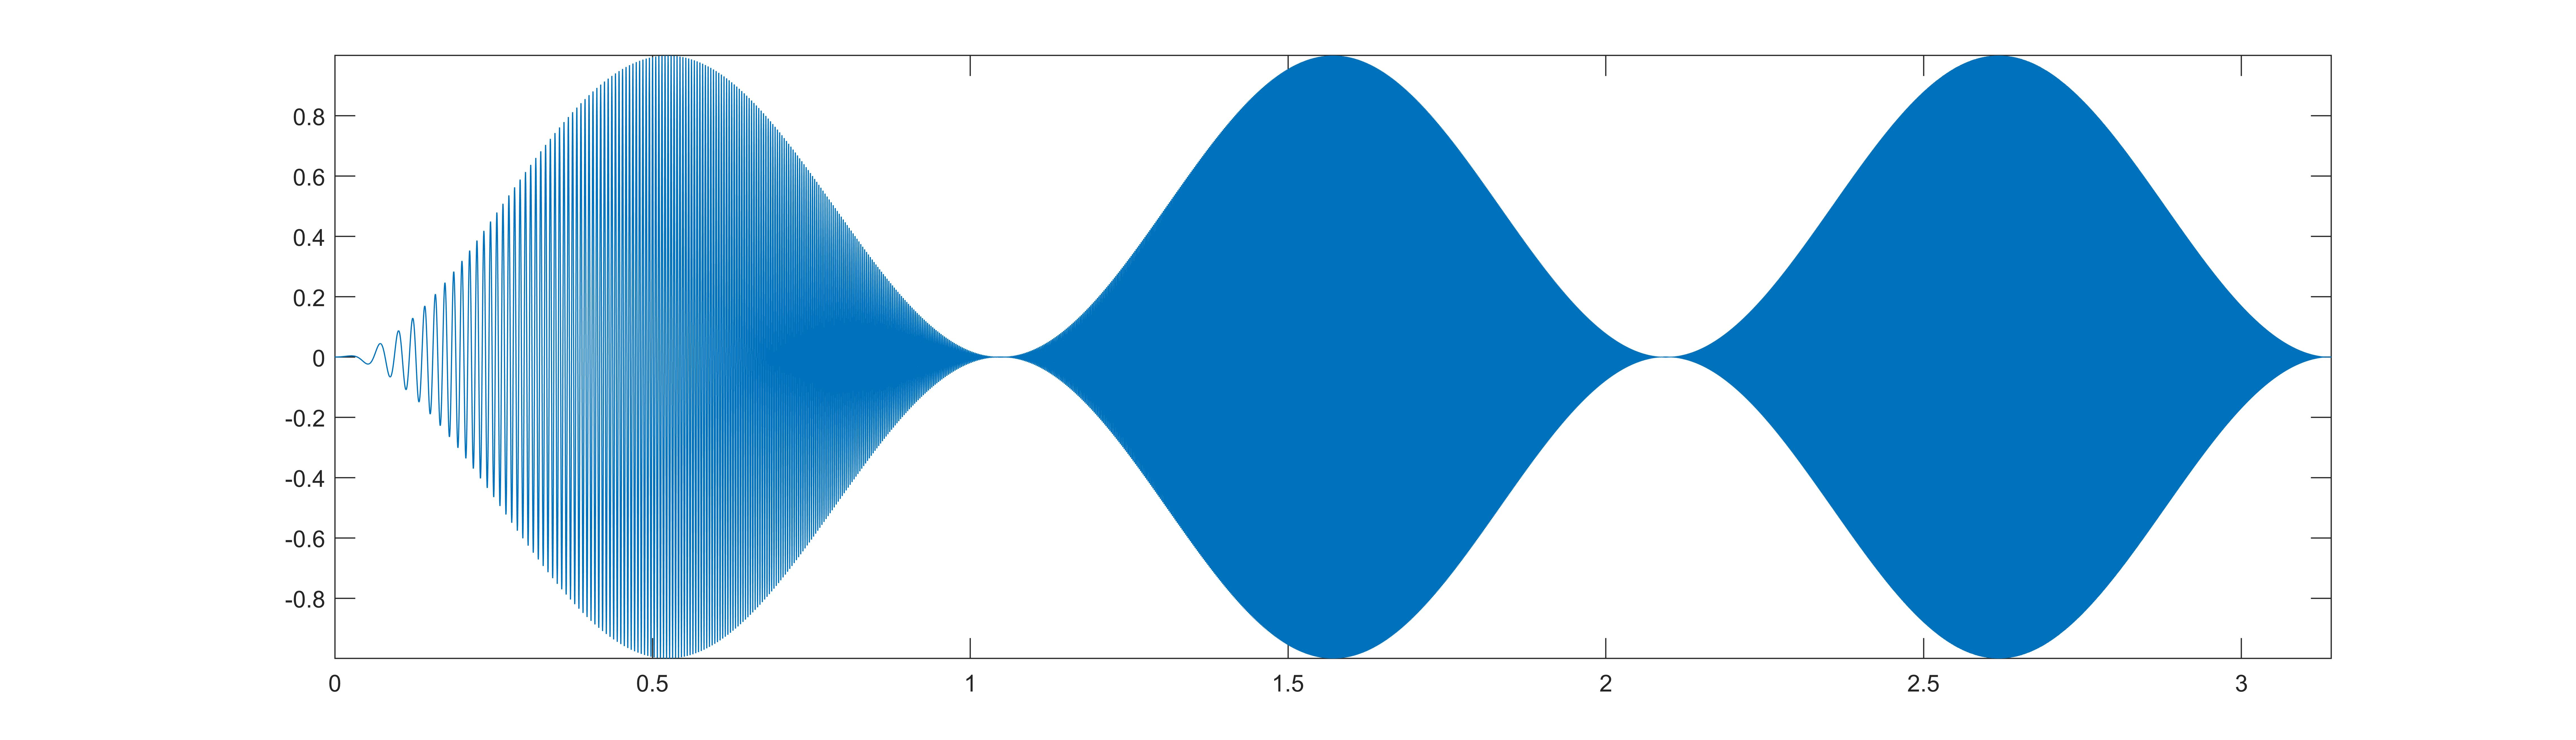
\includegraphics[width=\linewidth]{papers/autotune/sections/fft/signal.jpg}
	\captionof{figure}{Sweep Signal 0-400$Hz$}\label{fig:stftsig}
	\begin{tabularx}{\columnwidth}{XX}
		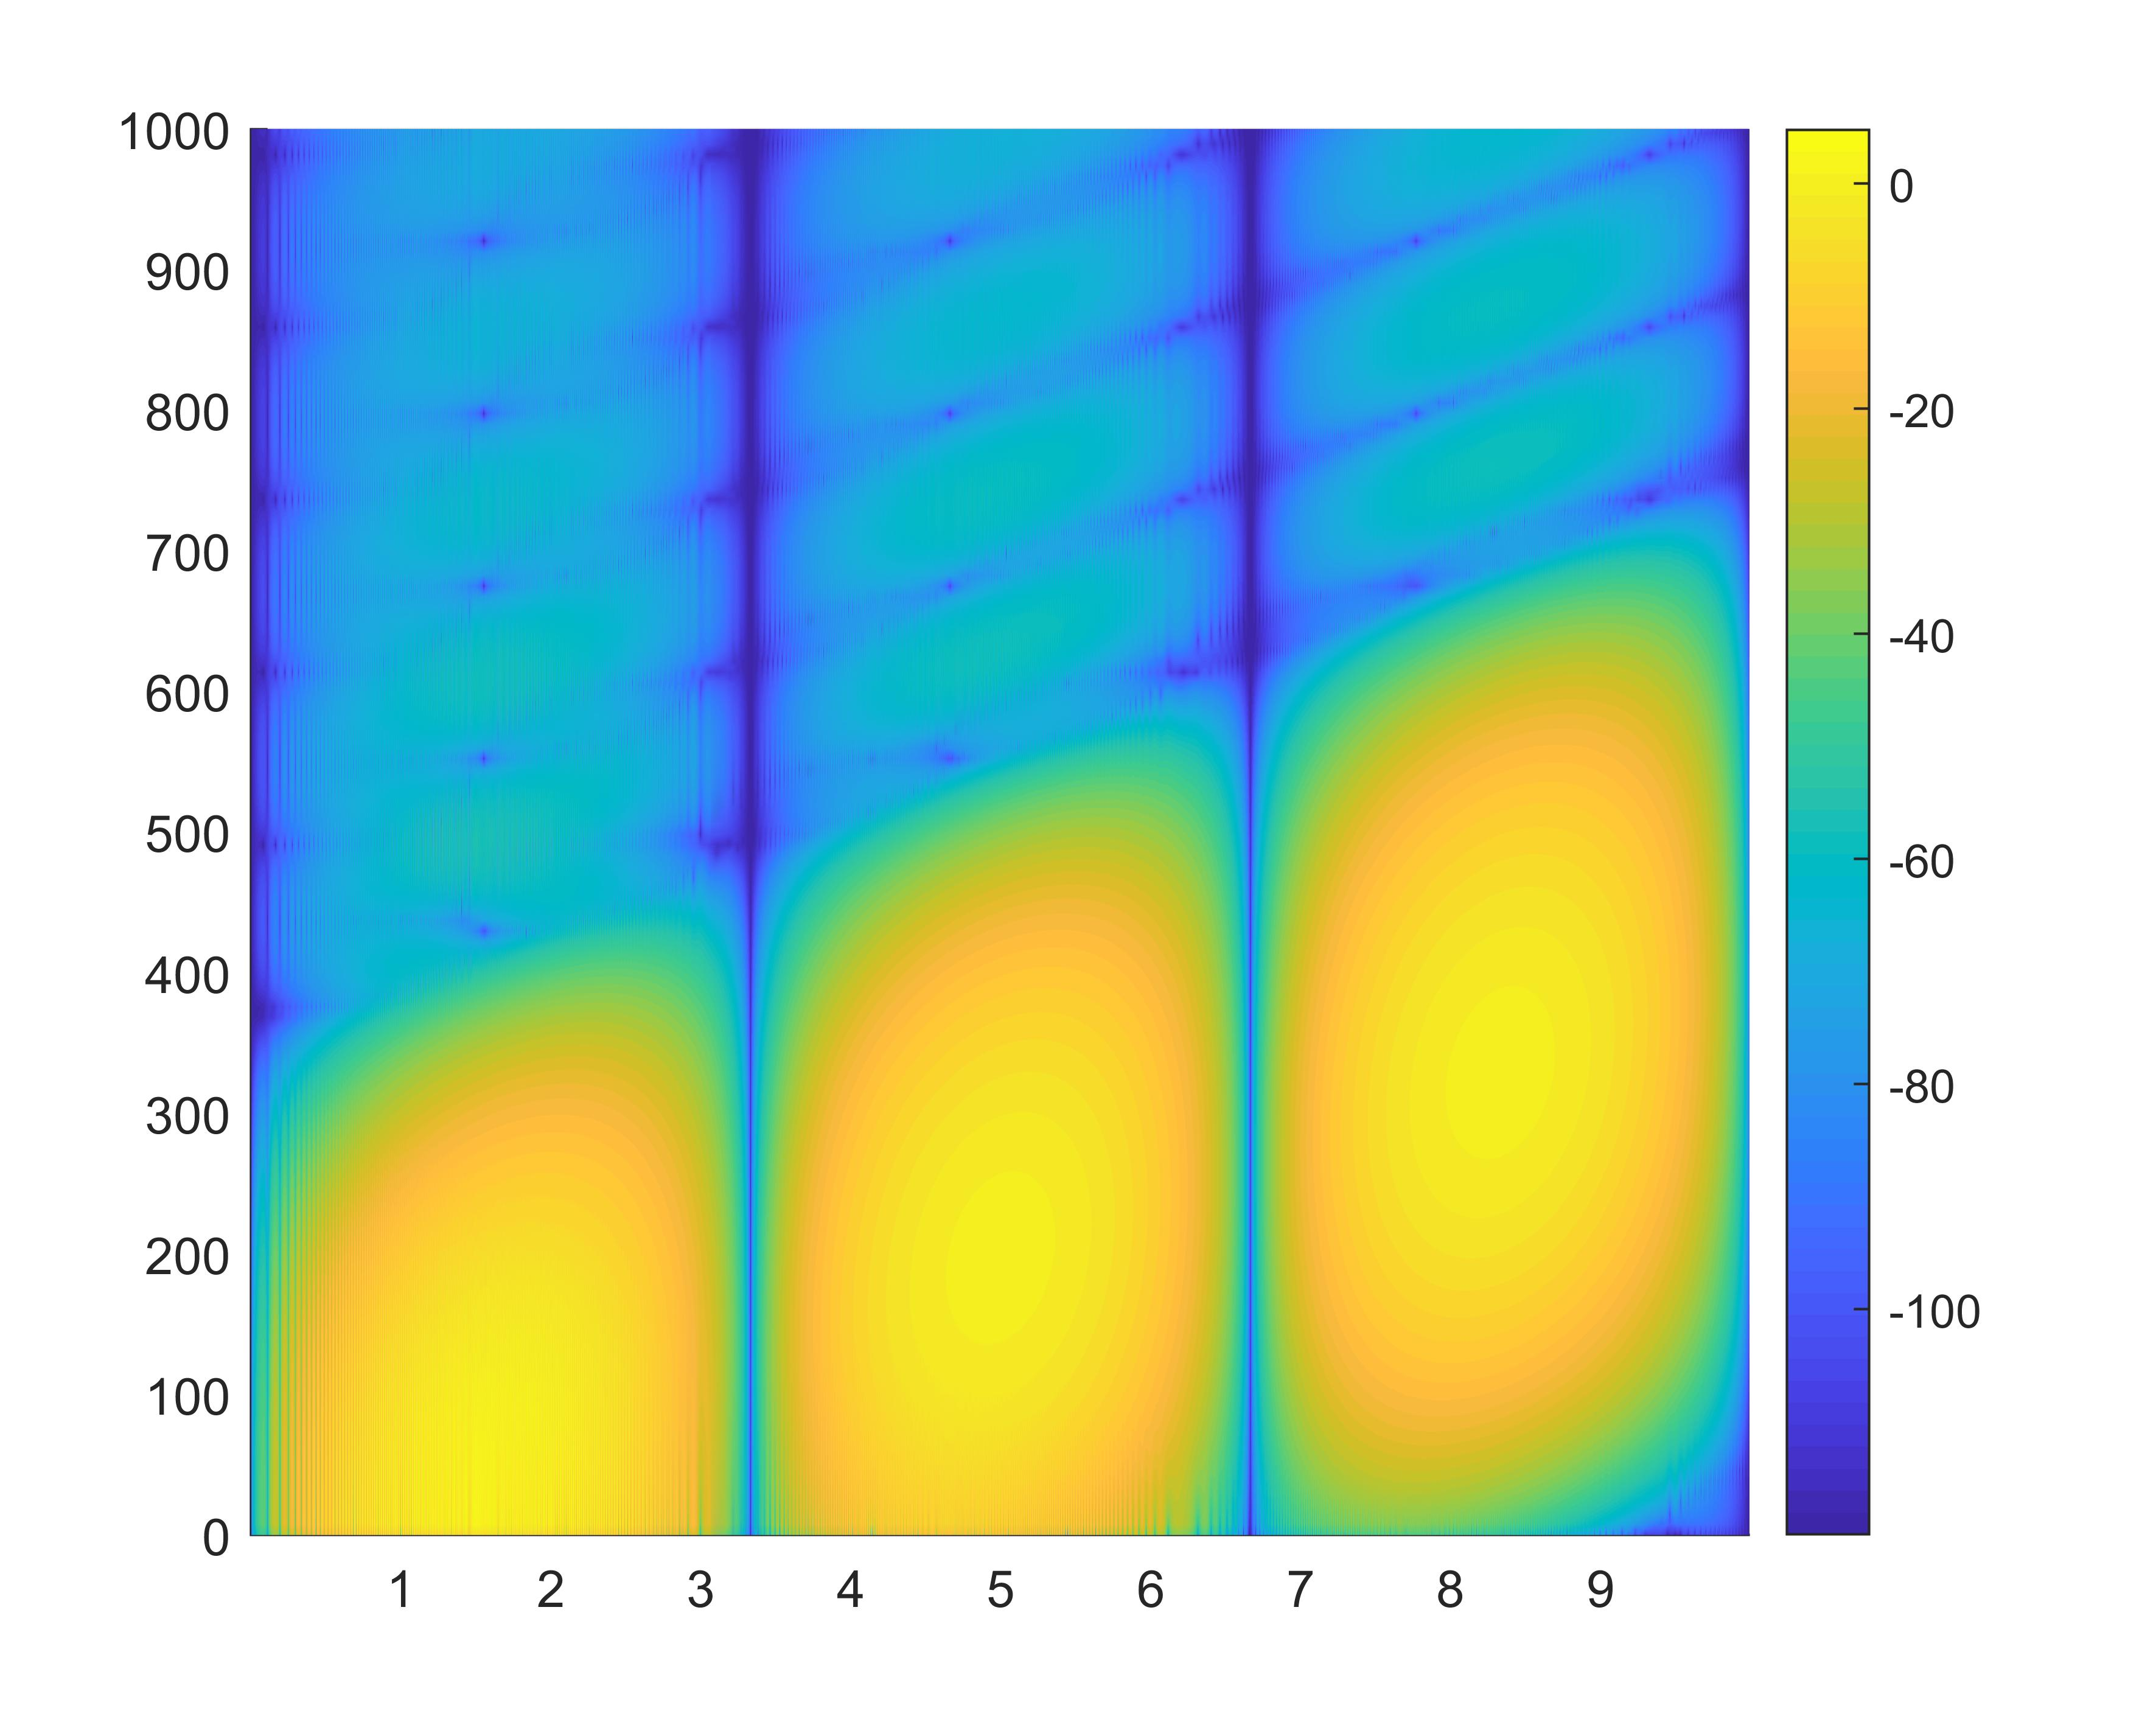
\includegraphics[width=\linewidth]{papers/autotune/sections/fft/stft256.jpg}
		\captionof{figure}{256 Sample Fenster}\label{fig:stft256}
		&   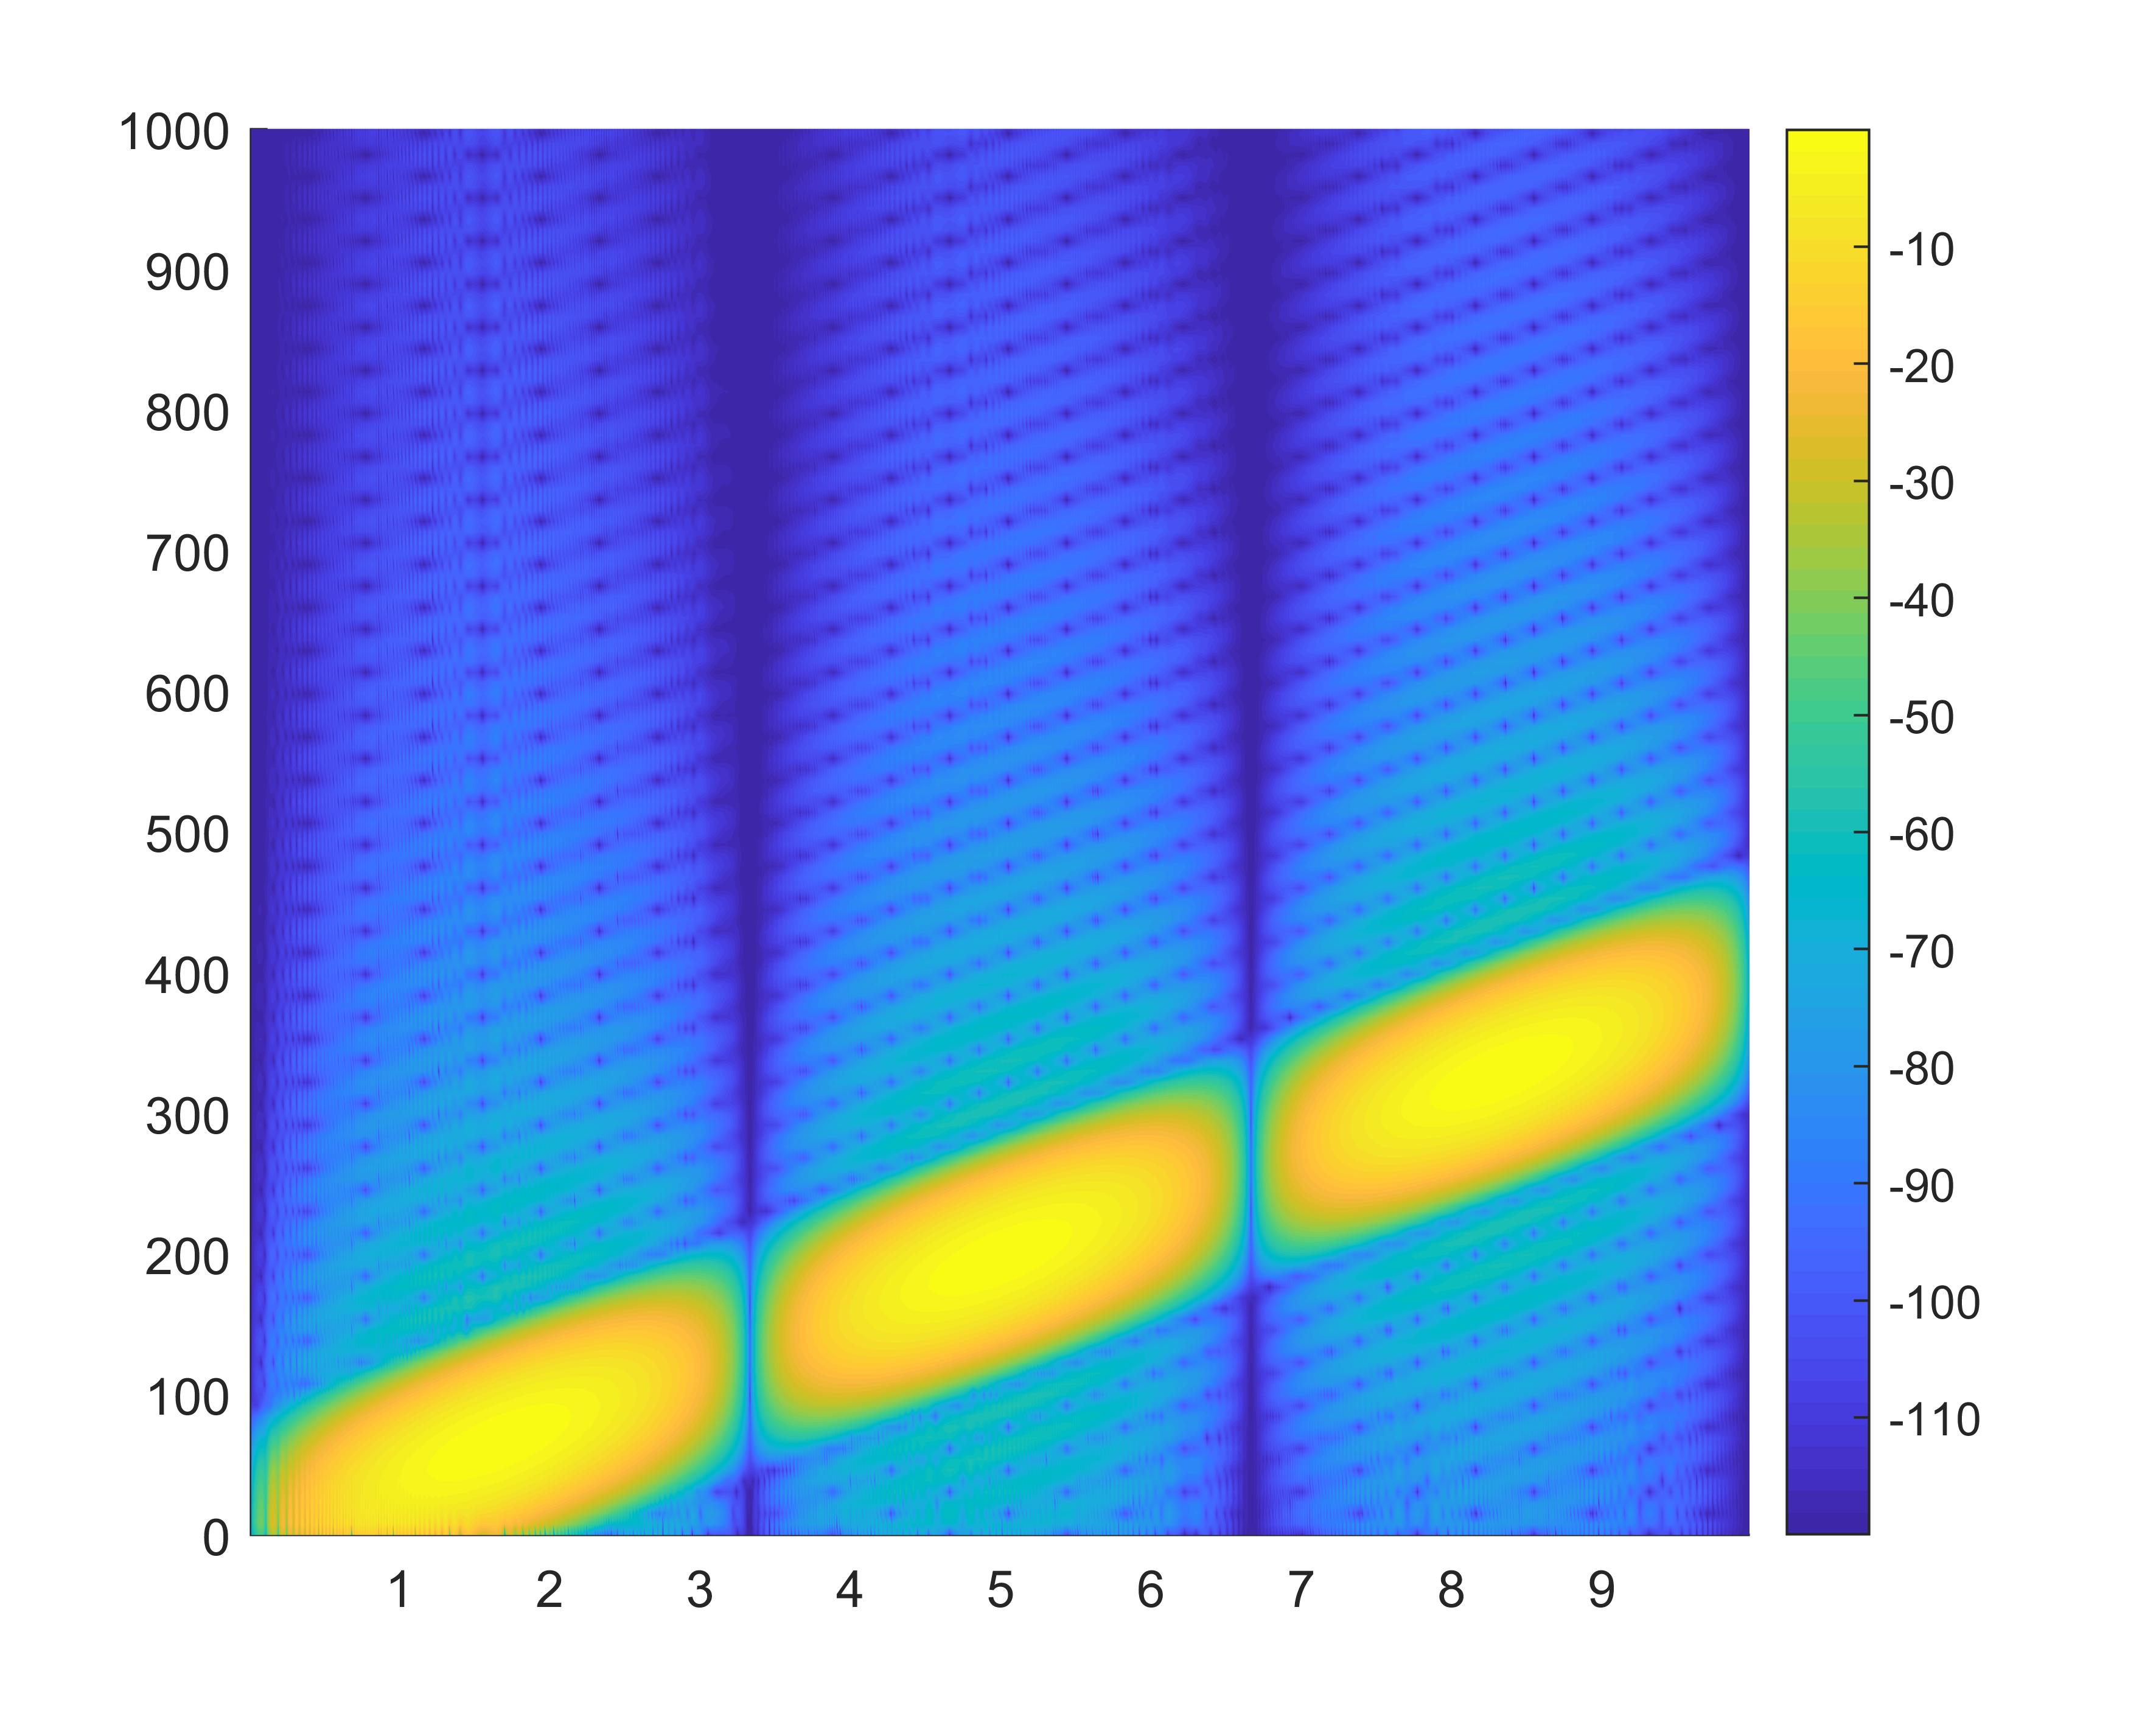
\includegraphics[width=\linewidth]{papers/autotune/sections/fft/stft1024.jpg}   
		\captionof{figure}{1024 Sample Fenster}\label{fig:stft1024}              \\    
		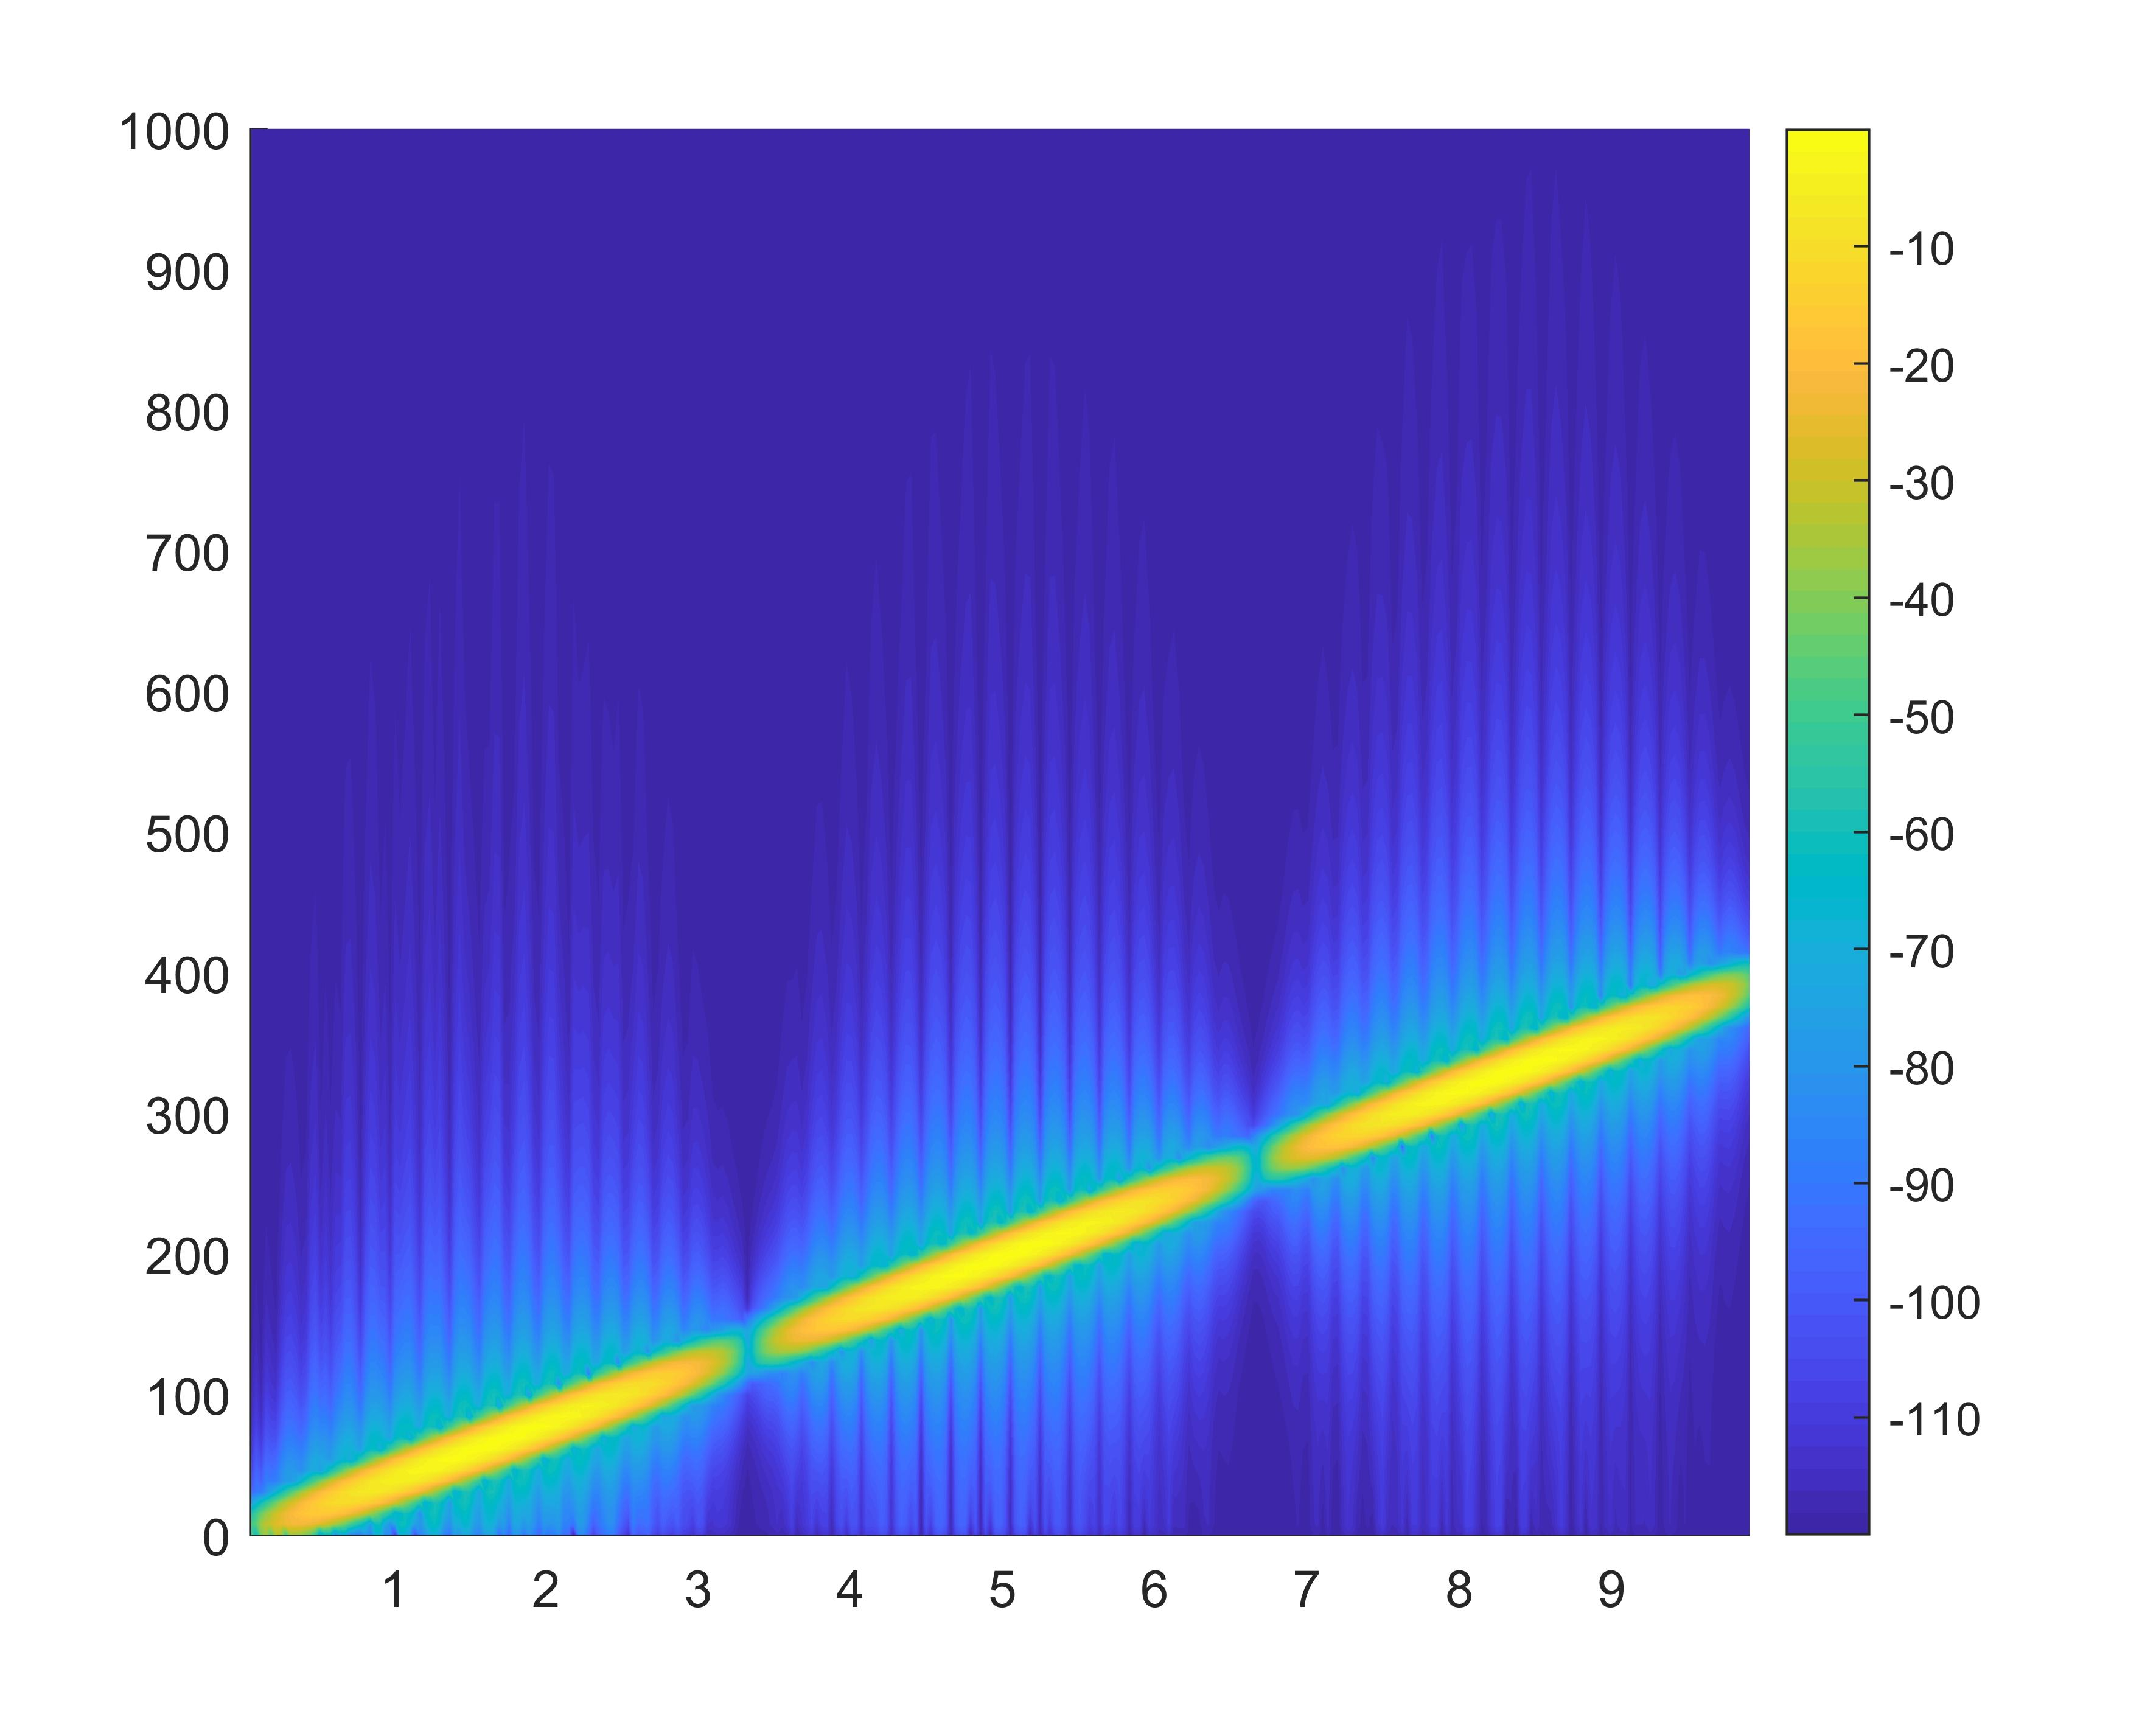
\includegraphics[width=\linewidth]{papers/autotune/sections/fft/stft4096.jpg}
		\captionof{figure}{4096 Sample Fenster}\label{fig:stft4096}
		&   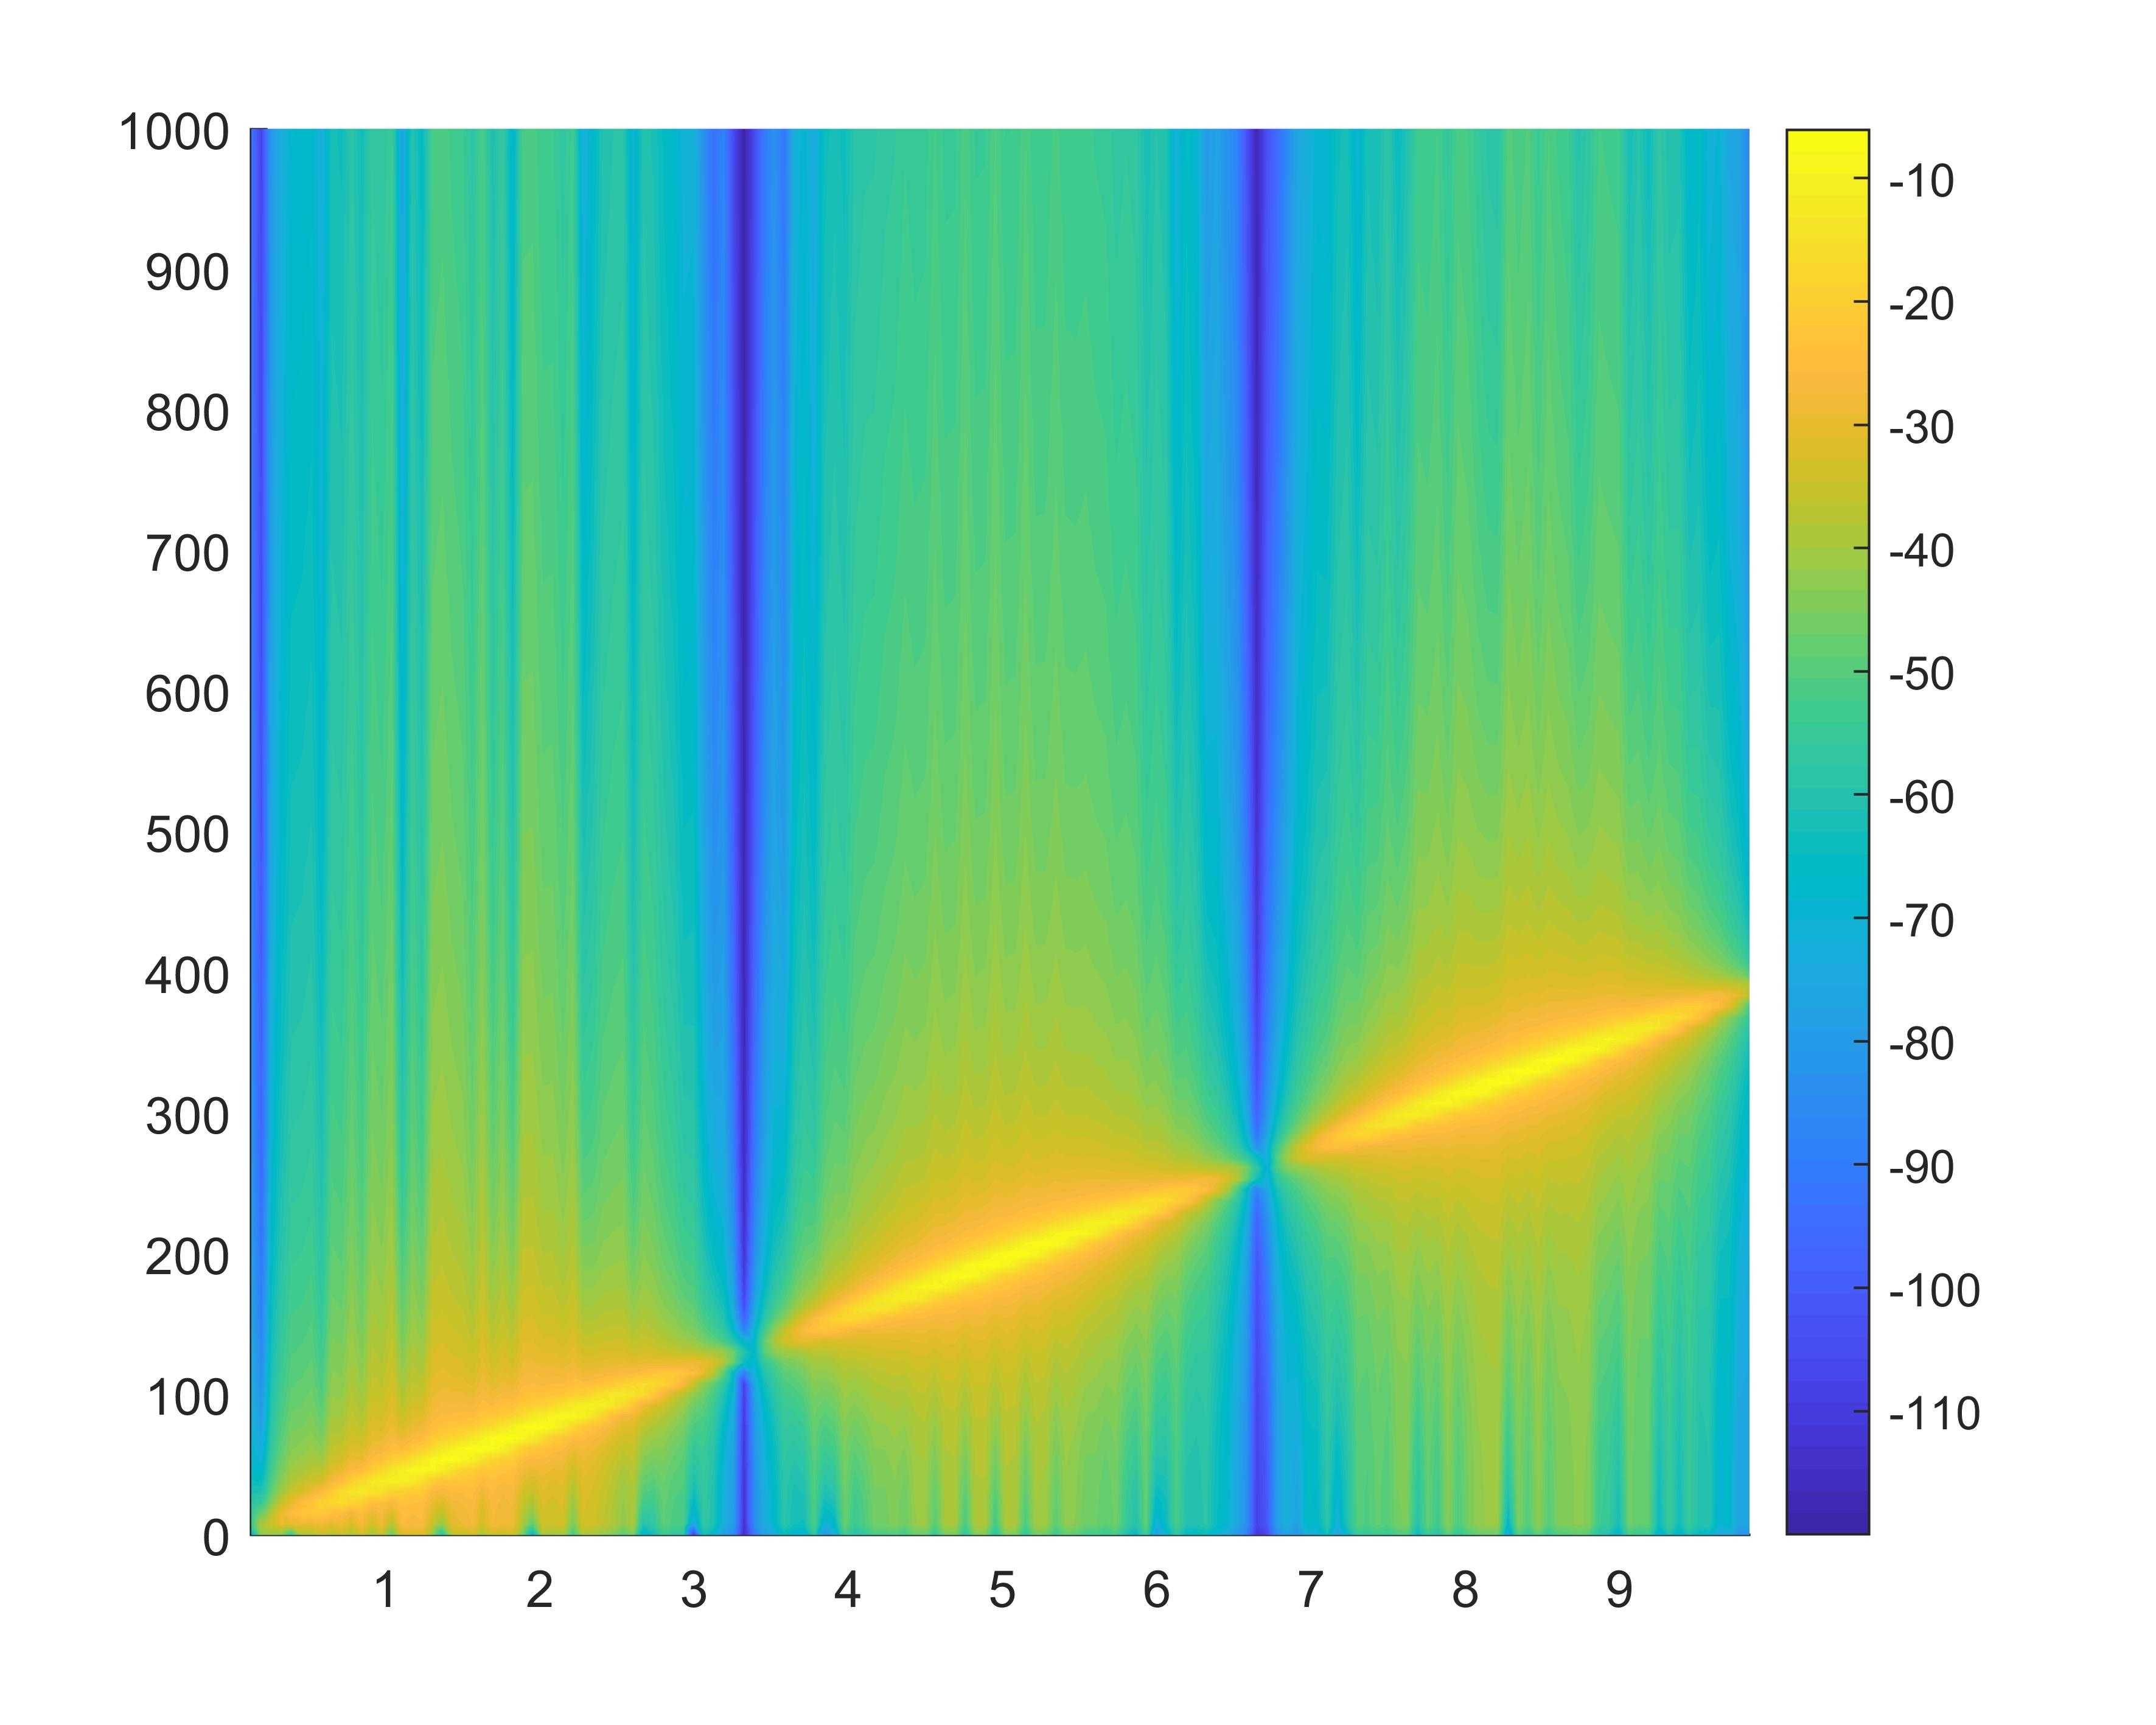
\includegraphics[width=\linewidth]{papers/autotune/sections/fft/stft8192.jpg}   
		\captionof{figure}{8192 Sample Fenster}\label{fig:stft8192}              \\           
	\end{tabularx}
	
	\caption{STFT}
	\label{tab:STFTtab}
\end{table}%


Wie man bei der Abbildung \ref{fig:stft256} gleich sieht ist die Streuung noch ernorm. Mann kann nur sehr grob wahrnehmen welche Frequenzen vorhanden sind. Dafür ist die Zeitliche Auflösung sehr gut mit einer scharfen Kante beim Nullpunkt. \\

Betrachtet man nun die Abbildung \ref{fig:stft1024} sind die Frequenzen schon viel deutlicher zu erkennen als bei einem Sampling von 256. Dafür wird in der Zeitlichen Auflösung ein wenig eingebüsst.\\

Das beste Bild ist bei 4096 Samples in der Abbildung \ref{fig:stft4096} zu sehen. Die Zeitliche abgrenzung verschwimmt ein wenig. Dafür ist die Frequenz deutlich ersichtlich.\\

In der Letzten Abbildung \ref{fig:stft8192} ist die zeit so langsam das die tiefen Frequenzen des Modultionssignal wieder einfluss nehmen auf das Spektogramm. Dies verfälscht das Resultat welches dann weniger brauchbar sein kann bei praktischen Auswertungen bei der die Modulationsfrequenz nicht so eine wichtige Rolle spielt.\\






